\chapter{Background}
\label{cha:background}

This chapter provides background for concepts used later in chapters~\ref{cha:impl-dynam-graph} and
\ref{cha:graph-track-prob}.  It gives a quick overview of Bayesian inference and probabilistic
programming in general, necessary to understand the requirements and usual approaches of
probabilistic programming systems.  Consequently, the machinery and language used to develop the
graph tracking system forming the main part of the work are described.  First, basic notions and
techniques of the Julia compilation process as well as the language's metaprogramming capabilities
are described, which form the basis of the implementation.  Second, a short introduction to graph
tracking and source-to-source automatic differentiation is given, from which many of the ideas and
terminology that will later be used were taken


%%%%%%%%%%%%%%%%%%%%%%%%%%%%%%%%%%%%%%%%%%%%%%%%%%%%%%%%%%%%%%%%%%%%%%%%%%%%%%%%%%%%%%%%%%%%%%%%%%%
\section{Bayesian Inference and MCMC methods}
\label{sec:bayes-infer}

Probabilistic modeling is an approach to model phenomena based on the assumption that observable
data can be fully described through some generative process that involves randomness.  Recovering
the details of this process, by estimating which one from a class of processes fits observed data
best, is a form of learning: if we have a good description of how observations are generated, we can
make summary statements about the whole population (descriptive statistics) or predictions about new
observations.  For example, learning the specifics a conditional relation between independently
observed paired data can be used to solve regression or classification problems.

Within the Bayesian framework, we assume that the generative process is specified by random
variables related through conditional distributions with densities, which describe how the
observables would be generated: some \emph{latent variables} are generated from \emph{prior
  distributions}, and the data are generated conditionally on the latent variables.  The goal is to
learn the \emph{posterior distribution} of the latent variables given the data.  Whereas the
generative model specifies how we assume data generation to work from latent to observed values in
\enquote{forward} direction, the posterior estimate allows us to reason \enquote{backwards} from
given observations to the latent values that have generated them.

As an example, consider image classification: if we assume that certain percentages of an image data
set picture cats and dogs, respectively, the distribution of these labels forms the prior.  Given
the information which kind of animal is depicted on it, an image can then be generated as a matrix
of pixels based on a distribution of images conditioned on labels.  The posterior distribution is
then conditional distribution of the label given an image.  When we have this information, we can,
for example, build a Bayesian classifier, by returning for a newly observed image that label which
has the highest probability under the posterior.\todo{Bayesian regression?}

In the following, we will mostly assume that the involved random variables have distributions with
respect to a suitable base measure, generally written as \(\mu\): the counting measure in the
discrete case, and the Lebesgue measure in the finite-dimensional continuous case
\parencite{kallenberg2006foundations}.  This allows to conveniently unify summation and integration
under one notation.  See chapter~\ref{ch:measure-theory} in the appendix for more information.

The posterior of the generative model can be expressed as a conditional distribution using Bayes'
theorem. In terms of densities, we then have\footnote{Note the abuse of notation regarding
  \(\prob{\cdot}\); see page~\pageref{cha:notation} on notation.}
\begin{equation}
  \label{eq:bayes}
  \overbrace{\prob{\theta \given x}}^{\text{posterior}} =
  \frac{\overbrace{\prob{x \given \theta}}^{\text{likelihood}}\;
    \overbrace{\prob{\theta}}^{\text{prior}}}{\prob{x}},
\end{equation}
where \(x\) are the observed data, and \(\theta\) are the latent values. The posterior represents
the distribution of the unobserved variables as a combination of the prior belief updated by what
has been observed~\parencite{congdon2006bayesian}.  \(\theta\) often functions as a parametrization
of the likelihood distribution.  Also note that in practice, one might not be interested in all of
the latent variables, but only a marginal; this corresponds to integrating out some parts of
\(\theta\).

Going beyond simple applications like the example mentioned above, handling the posterior gets
difficult, though.  Simply evaluating the posterior density
\(\theta \mapsto \prob{\theta \given x}\) at single points is not enough in a Bayesian setting for
usages such as prediction, certain parameter estimation methods, or exact evaluation of the
normalization term \(\prob{x}\).  The problem is that almost all of the relevant quantities depend
on some sort of expectation over the posterior, an integral of the form
\begin{equation}
  \label{eq:posterior-expectation}
  \Exp{f(\Theta) \given X = x} = \int f(\theta) \prob{\theta \given x} \dif \mu(\theta),
\end{equation}
for some (measurable) function \(f\). This in turn involves calculating the marginal
\begin{equation}
  \label{eq:normalizing}
  \prob{x} = \int \prob{x, \theta} \dif \mu(\theta),
\end{equation}
the normalization term in equation~\eqref{eq:bayes}, often called the \enquote{model evidence}.

When the involved distributions are of a sufficiently \enquote{nice} form, e.g., a conjugate pair
\parencites[see][chapter 2.2.2]{marin2007bayesian}[chapter 9.2.5]{murphy2012machine}, the
integration can be performed analytically, since the posterior density has a closed form for a
certain known distribution, or at least is a known integral.  In general, however, this is not
tractable, not even by standard numerical integration methods, and approximations have to be made.
Even for discrete variables, naive application of summation can lead to combinatorial explosion.

\newthought{Different techni{q}ues} for posterior approximation are available: among them are
optimization-based approaches for general graphical models, such as variational inference
\parencite[chapter 21 and 22]{murphy2012machine} and other methods generalized under the framework
of message passing \parencite{minka2005divergence}.  The methods described in this thesis, however,
fall into the category of Monte Carlo methods, and are based on sampling \parencites[chapter
23]{murphy2012machine}{vihola2020lectures}.  Their fundamental idea is to derive, for given
observations \(x\) and a specified density of \(\Theta \from \pi(\cdot \given x)\), a sampling
procedure with a consistent estimator for expectations:
\begin{equation}
  \label{eq:mc-methods}
  \kth{I}(f) \to \Exp{f(\Theta) | X = x} = \int f(\theta) \pi(\theta \given x) \dif\mu(\theta), \quad \text{as} \quad k
  \to \infty
\end{equation}
in some appropriate stochastic convergence (usually convergence in probability is enough).

Examples of such methods are rejection sampling \parencites[chapter
II.3]{devroye1986nonuniform}[section 4]{vihola2020lectures}, importance sampling \parencite[section
4]{vihola2020lectures}, and particle filters \parencite{dahlin2015getting}.  Many Monte Carlo
methods are defined in a form that directly samples a sequence of individual random variables
\(\sequence{\kth{Y}}\), called a \emph{chain}, for which the estimator is given by the arithmetic
mean, such that a law of large numbers (LLN) holds:
\begin{equation}
  \label{eq:mc-lln}
  \kth{I}(f) = \frac{1}{k} \sum_{i=1}^{k} f(\kth[i]{Y}) \to \Exp{f(\Theta) \given X = x}
\end{equation}
If we can sample \(\kth{Y} \from \pi(\cdot \given x)\) exactly, they are \iid{} and the LLN holds
trivially; such samplers exist, but might also be difficult to derive or not possess good enough
convergence properties (especially in high dimensions).  Another large class of samplers is formed
by \emph{Markov Chain Monte Carlo} (MCMC) methods \parencite{vihola2020lectures,robert1999monte},
which, instead of sampling exactly from the density, define \(\kth{Y}\) via a (time-homogeneous)
Markov chain:
\begin{equation}
  \label{eq:mc-kernel}
  \begin{aligned}
    &\Prob{\kth[k+1]{Y} \in \dif y
      \given \kth{Y} = \kth{y}, \ldots, \kth[1]{Y} = \kth[1]{y}} \\
    &\quad = \Prob{\kth[k+1]{Y} \in \dif y \given \kth{Y} = \kth{y}}  \\
    &\quad = K(\kth{y}, \dif y) \\
    % &\quad = k(y \given \kth{y}) \dif\mu(y)
  \end{aligned}
\end{equation}
for all \(k \ge 1\).  By constructing the parameterized measure \(K\), the \emph{transition kernel},
in the right way, the resulting has target density \(\pi(\cdot \given x)\) as the unique stationary
distribution~-- that means for all \(\pi(\cdot \given x)\)-measurable sets \(A\),
\begin{equation}
  \label{eq:stationarity}
  \int \pi(\theta \given x) K(\theta, A) \dif\mu(\theta) = \int_A \pi(\theta \given x) \dif\mu(\theta) =
  \Prob{\Theta \in A \given X = x},
\end{equation}
and the LLN for Markov chains holds.  (For discrete spaces, this relation is more familiarly written
as a left eigen-problem on a stochastic matrix: \(\pi K = \pi\) for \(x\) fixed, and \(\pi\) and
\(K\) considered a vector and matrix.)  The advantage of MCMC methods is that they apply equally
well to many structurally complex models, and treat densities in a uniform way, without requiring
special knowledge about the specific distribution in question.  I refer to \textcites[chapter
6]{vihola2020lectures}{robert1999monte}[chapters 24 and following]{murphy2012machine} as
introductions to MCMC theory practice.

\newthought{Fre{q}uently, MCMC methods} are variations of the \emph{Metropolis-Hastings algorithm}
(MH), which splits the general definition of the transition kernel into two parts: a proposal
distribution, given by a transition kernel
\((\kth[k-1]{y}, \kth{y}) \mapsto q(\kth[k-1]{y}, \kth{y})\) which is easy to sample from, and an
acceptance rate function \(\alpha\).  Subsequent samples are then produced by proposing values from
the conditional distribution \(q(\kth[k-1]{y}, \cdot)\) dependent on previous chain element
\(\kth[k-1]{y}\), and incorporating them into the chain with a probability given through \(\alpha\)
(see algorithm~\ref{alg:mh}).  There exist many MH-based schemes with different properties and
requirements: from the classical random-walk Metropolis algorithm with Gaussian proposals, over
Reversible Jump MCMC for varying dimensions \parencite{green1995reversible}, to gradient-informed
methods like Metropolis Adjusted Langevin and Hamiltonian Monte Carlo (HMC)
\parencite{betancourt2018conceptual,girolami2011riemann}.

% \begin{algorithm}[t]
%   \sffamily
%   \hrule
%   \begin{enumerate}
%     \firmlist
%   \item Start from an arbitrary \(\kth[1]{Y} = \kth[1]{y}\) with \(\pi(\kth{y}) > 0\).
%   \item For each \(k \ge 1\):
%     \begin{enumerate}
%       \firmlist
%     \item Sample a proposal \(\kth[k]{\hat{Y}} \from q(\kth[k-1]{Y}, \cdot)\).
%     \item With probability \(\alpha(\kth[k]{\hat{Y}}, \kth[k-1]{Y})\), set
%       \(\kth[k]{Y} = \kth[k]{\hat{Y}}\); else, keep \(\kth[k]{Y} = \kth[k-1]{Y}\).
%     \end{enumerate}
%   \end{enumerate}
%   \hrule
%   \caption{General scheme for the Metropolis-Hastings algorithm.\label{alg:mh}}
% \end{algorithm}

\begin{algorithm}[t]
  \hrule
  \begin{algorithmic}
    \State Start from an arbitrary \(\kth[1]{Y} = \kth[1]{y}\) with \(\pi(\kth{y}) > 0\)
    \For{\(k \ge 1\)}
    \State Sample a proposal \(\kth[k]{\hat{Y}} \from q(\kth[k-1]{Y}, \cdot)\)
    \State With probability \(\alpha(\kth[k]{\hat{Y}}, \kth[k-1]{Y})\), set
    \(\kth[k]{Y} = \kth[k]{\hat{Y}}\); else, keep \(\kth[k]{Y} = \kth[k-1]{Y}\)
    \EndFor
  \end{algorithmic}
  \hrule
  \caption{General scheme for the Metropolis-Hastings algorithm.\label{alg:mh}}
\end{algorithm}

For multi-component structures, where the latent variables have a blocked form
\(\Theta = [\Theta_1, \ldots, \Theta_M]\), a good proposal distribution can be hard to find, though.
One way to break down the problem is to use a family of block-wise updates, given by conditional
kernels \(q_{i}\) operating on only the \(i\)-th block of \(\Theta\), with the others fixed.  Then
we can use the following modified proposal \(\hat{Y}\) in algorithm~\ref{alg:mh},
\begin{equation}
  \label{eq:conditional-kernels}
  \begin{aligned}
    \kth[k]{\hat{Y}}_{-i} &= \kth[k-1]{Y}_{-i}, \\
    \kth[k]{\hat{Y}}_{i} &\from q_{i}(\kth[k-1]{Y}_{i}, \cdot \given \kth[k-1]{Y}_{-i})
  \end{aligned}
\end{equation}
(notable independent of the previous \(\kth[k-1]{y}_{i}\)).  The blocks can be scalar or
multivariate, the kernels may themselves be any valid transition kernel, and the order of the blocks
\(i\) can be chosen in different random or determinstic ways under some technical conditions
\parencite[chapter 6.6]{vihola2020lectures}.  This allows one to freely mix different MCMC methods
suitable for each variable in a problem.

This so-called \enquote{within-Gibbs} sampler bears its name because it is a generalization of the
classical \emph{Gibbs sampling} algorithm \parencite{geman1984stochastic}, using as a simple set of
transition kernels the conditional distributions:
\begin{equation}
  \label{eq:gibbs-conditional-kernel}
  q_{i}(\kth[k-1]{y}_{i}, \dif \kth{y}_{i} \given \kth[k-1]{y}_{-i}) =
  \Prob{\kth{\Theta}_{i} \in \dif\kth{y}_{i} \given \kth[k-1]{\Theta}_{-i} = \kth[k-1]{y}_{-i}}.
\end{equation}
They can directly be used as component proposals for a within-Gibbs sampler, leading to a canceling
acceptance rate of \(\alpha \equiv 1\).  This approach has the advantage of being very algorithmic,
which makes it rather easy to apply, even by hand, to many models.  Hence, the method is a popular
starting point for general probabilistic programming systems, most prominently BUGS
\parencite{lunn2000winbugs,lunn2009bugs} and JAGS \parencite{plummer2003jags,plummer2017jags}.

In many real-world models, the factorization structure is quite sparse and results in small Markov
blankets.  Algorithms to derive Gibbs samplers exploit this large independency between variables.
In short, they \enquote{trim} the dependency graph of the model to the local Markov blankets of each
target variable, and derive either a full conditional from it, where possible (for discrete or
conjugate variables), or otherwise approximate it through appropriate local sampling (e.g., slice
sampling) \parencite[see][]{plummer2003jags}.

As an example, consider a simple Gaussian mixture model with equal weights, specified as follows:
\begin{equation}
  \label{eq:normal-mixture-1}
  \begin{aligned}
    \mu_{k} &\iidfrom \Normal(m, s) \quad\text{for } 1 \le k \le K, \\
    Z_{n} &\iidfrom \distr{Categorical}(K) \quad\text{for } 1 \le n \le N, \\
    X_{n} &\iidfrom \Normal(\mu_{Z_{n}}, \sigma) \quad\text{for } 1 \le n \le N.
  \end{aligned}
\end{equation}
To derive the conditional distribution of \(Z_{n}\) given the remaining variables, we start by
writing down the factorization of the joint density:
\begin{equation}
  p(z_{1:N}, \mu_{1:K}, x_{1:N}) = \prod_{k} p(\mu_{k}) \prod_{n} p(z_{n}) \prod_{n} p(x_{n} | \mu_{z_{n}}).
\end{equation}
From this, we can derive an unnormalized density proportional to the conditional by removing all
factors not including the target variable:
\begin{equation}
    p(z_{n} \given z_{-n}, \mu_{1:K}, x_{1:N}) \propto p(z_{n}) p(x_{n} | \mu_{z_{n}})
\end{equation}
This is equivalent to finding the Markov blanket of \(Z_{n}\): only those conditionals relating the
target variable to its children and parents remain.  Since the clusters are drawn from a categorical
distribution, the support is discrete, and we can find the normalization constant by summation:
\begin{equation}
  \setlength{\jot}{0.8\baselineskip}
  \begin{aligned}
    &p(z_{n} \given z_{-n}, \mu_{1:K}, x_{1:N}) \\
    % &\quad = p(z_{n}) p(x_{n} | \mu_{z_{n}}) / Z \\
    &\quad = \dfrac{\distr{Categorical}(z_{n} \given K) \, \Normal(x_{n} \given \mu_{z_{n}}, \sigma)}{
      \sum_{k \in\, \supp(Z_{n})} \distr{Categorical}(k \given K)\, \Normal(x_{n} \given \mu_{k},
      \sigma)}, \\
    % &\quad = \dfrac{\distr{Categorical}(z_{n} \given K) \, \Normal(x_{n} \given \mu_{z_{n}}, \sigma)}{
    %   \sum_{k = 1}^{K} \distr{Categorical}(k \given K)\, \Normal(x_{n} \given \mu_{k}, \sigma)},
  \end{aligned}
\end{equation}
which can be expressed as a general discrete distribution over \(\supp(Z_{n}) = \{1, \ldots, K\}\),
with the unnormalized weights given by the numerator.  Next, the conditionals of the \(\mu_{k}\)
have the form
\begin{equation}
  \setlength{\jot}{0.8\baselineskip}
  \begin{aligned}
    &p(\mu_{k} \given z_{1:N}, \mu_{-k}, x_{1:N}) \\
    &\quad \propto p(\mu_k) \prod_{n} p(x_{n} | \mu_{k})^{\indicator{z_{n} \, = \, k}} \\
    &\quad = \prod_{n} \left( \Normal(\mu_{k} \given m, s) \,
      \Normal(x_{n} \given \mu_{k}, \sigma) \right)^{\indicator{z_{n} \, = \, k}}
  \end{aligned}
\end{equation}
which we recognize as a product of conjugate pairs of normal distributions.  More examples are
extensively covered in \textcite[chapter 24.2]{murphy2012machine}.

%%%%%%%%%%%%%%%%%%%%%%%%%%%%%%%%%%%%%%%%%%%%%%%%%%%%%%%%%%%%%%%%%%%%%%%%%%%%%%%%%%%%%%%%%%%%%%%%%%%
\section{Probabilistic Programming}
\label{sec:prob-prog}

\begin{lstfloat}
  \begin{lstlisting}[style=lstfloat]
@model function normal_mixture(x, K, m, s, σ)
    N = length(x)

    μ = Vector{Float64}(undef, K)
    for k = 1:K
        μ[k] ~ Normal(m, s)
    end

    z = Vector{Int}(undef, N)
    for n = 1:N
        z[n] ~ Categorical(K)
    end

    for n = 1:N
        x[n] ~ Normal(μ[z[n]], σ)
    end

    return x
end
\end{lstlisting}
    \caption{\turingjl{} implementation of a Gaussian mixture model with prior on the cluster centers,
    equal cluster weights, and all other parameters fixed.\label{lst:normal}}
\end{lstfloat}

Probabilistic programming is a structured way implementing generative models, as described in the
previous section, through the syntax of a programming language.  It is beneficial to consider
probabilistic programs not only as syntactic sugar for denoting the implementation of a joint
probability density over some set of variables, but as organized objects in their own right: they
open up possibilities that \enquote{black box} density functions cannot automatically provide. In
more concise terms of \textcite{vandemeent2018introduction}:
\begin{quote}
  Probabilistic programming is largely about designing languages, interpreters, and compilers that
  translate inference problems denoted in programming language syntax into formal mathematical
  objects that allow and accommodate generic probabilistic inference, particularly Bayesian
  inference and conditioning.
\end{quote}

A probabilistic program differs from a regular program (that may also contain stochastic parts)
through the possibility of being conditioned on: some of the internal variables can be fixed to
observed values, from outside. As such, the program denotes on the one hand a joint distribution,
that can be \emph{forward sampled} from by simply running the program top to bottom and producing
(pseudo-) random values.  But at the same time, it also represents a conditional distribution, in
form on the unnormalized conditional density, which together with an inference algorithm can also be
\emph{backward sampled} from.  (Other terms, such as \enquote{evaluation} and \enquote{querying},
are used as well.)  Consider the model~\eqref{eq:normal-mixture-1} from above: to perform inference
on it in \turingjl{} \parencite{ge2018turing}, the probabilistic programming language used in this
thesis, its mathematical description might be translated into the Julia program given in
listing~\ref{lst:normal}.

We can then sample from the model in several ways using Julia:
\begin{lstlisting}
julia> m = normal_mixture(x_observations, K, m, s, σ);
julia> forward = sample(m, Prior(), 10);
julia> chain = sample(m, MH(), 1000);
\end{lstlisting}
The value of \jlinl{forward} will be an dataframe-like object containing 10 values for each variable
sampled from the forward (i.e., joint) distribution, matching the size of \jlinl{x_observations}.
Similarly, \jlinl{chain} will contain a length 1000 sample from a Markov chain targeting the
posterior, conditionally on \jlinl{x_observations}, created using the MH algorithm.  If we were to
write out code for these two functionalities manually, in idiomatic Julia, we would end up with at
least two separate functions needed for the sampler:
\begin{lstlisting}
function normal_mixture_sampler(N, K, m, s, σ)
    μ = rand(Normal(m, s), K)
    z = rand(Categorical(K), N)
    x = rand.(Normal.(μ[z], s))
    return μ, z, x
end

function normal_mixture_logpdf(μ, z, x, K, m, s, σ)
    N = length(x)
    ℓ = 0.0
    ℓ += sum(logpdf(Normal(m, s), μ[k]) for k = 1:K)
    ℓ += sum(logpdf(Categorical(K), z[n]) for n = 1:N)
    ℓ += sum(logpdf(Normal(μ[z[n]]), x[n]) for n = 1:N)
    return ℓ
end
\end{lstlisting}
And still, with these, we would lack much of the flexibility that models written in \turingjl: no
general interface for sampling algorithms to automatically detect all latent and observed variables;
no possibility for other, nonstandard execution forms as are needed for Variational Inference or
gradient computation for HMC; no automatic name extraction and dataframe building for chains.  All
these points highlight the advantages of dedicated probabilistic programming languages (PPLs) over
hand-written model code.  (Additionally, there is of course a benefit of reducing errors introduced
by the sampling function not matching the likelihood function, or errors involving
log-probabilities.)

\newthought{Many PPLs are implemented} as external domain-specific languages (DSLs), like Stan
\parencite{carpenter2017stan}, JAGS \parencite{plummer2003jags}, and BUGS
\parencite{lunn2000winbugs,lunn2009bugs}.  Others are specified in the \enquote{meta-syntax} of Lisp
S-expressions, as Church \parencite{goodman2012church}, Anglican \parencite{wood2015new}, or Venture
\parencite{mansinghka2014venture}.  A third group is embedded into host programming languages with
sufficient syntactic flexibility, for example \juliapackage{Gen.jl}
\parencite{cusumano-towner2019gen,cusumano-towner2020gen} and \juliapackage{Soss.jl}
\parencite{scherrer2019soss} in Julia (besides the already named \turingjl{}), or Pyro
\parencite{bingham2018pyro} and PyMC3 \parencite{salvatier2016probabilistic} in Python.

The latter approach is advantageous when one wants to enable the use of regular, general-purpose
programming constructs or interact with other functionalities of the host language.  There are also
a variety of further reasons why one would rather describe an inference problem in terms of a
program than in more \enquote{mathematical} form, like as a graph or likelihood function.  In a good
probabilistic programming DSL, models will read as close to textbook model specifications as
possible, while allowing to use the host language to:
\begin{itemize}
  % \firmlist
\item define recursive relationships,
\item write models using imperative constructs, such as loops, or mutable intermediate computations
  for efficiency,
\item optimize details of the execution, e.g. for memoization, likelihood scaling, or preliminary
  termination,
\item use distributions over complex custom data structures, e.g. trees,
\item perform inference involving complex transformations from other domains, for which
  implementations already exist, e.g. neural networks or differential equation solvers , or
\item integrate calls to very complex external systems, e.g. simulators or renderers.
\end{itemize}
Depending on the choice of features should be supported, several possibilities for the
implementation of such a DSL exist.  All are based on some form of abstract interpretation.  A rough
distinction can be made between \emph{compilation-based methods}, which statically translate the
model code to a graph or density function, and \emph{evaluation-based methods}, which dynamically or
implicitly build such a structure at run-time, by allowing an inference algorithm to interleave the
execution.  The latter make it easier to include host-language control constructs.  See
\textcite{vandemeent2018introduction} for a general introduction into some common implementation
approaches for PPLs, and \textcite{goodman2014design} for a detailed overview of the internals of
one specific, continuation-based implementation called WebPPL (using a Lisp-based syntax).

\begin{lstfloat}
  \begin{lstlisting}[style=lstfloat]
function normal_mixture(x, K, m, s, σ)
    function evaluator(rng, model, varinfo, sampler, context, x, K, m, s, σ)
        N = length(x)
        μ = Vector{Float64}(undef, K)
        for k = 1:K
            dist_mu = Normal(m, s)
            vn_mu = @varname μ[k]
            inds_mu = ((k,),)
            μ[k] = tilde_assume(
                rng, context, sampler, dist_mu, vn_mu, inds_mu, varinfo
            )
        end
        z = Vector{Int}(undef, N)
        for n = 1:N
            dist_z = Categorical(K)
            vn_z = @varname z[n]
            inds_z = ((n,),)
            z[n] = tilde_assume(
                rng, context, sampler, dist_z, vn_z, inds_z, varinfo
            )
        end
        for n = 1:N
            dist_x = Normal(μ[z[n]], σ)
            vn_x = @varname(x[n])
            inds_x = ((n,),)
            if isassumption(model, x, vn_x)
                x[n] = tilde_assume(
                    rng, context, sampler, dist_x, vn_x, inds_x, varinfo
                )
            else
                tilde_observe(
                    context, sampler, dist_x, x[n], vn_x, inds_x, varinfo
                )
            end
        end
        return x
    end
    return Model(
        :normal_mixture, evaluator, 
        (x = x, K = K, m = m, s = s, σ = σ), 
        NamedTuple()
    )
end
\end{lstlisting}
  \caption{Slightly simplified macro-expanded code of the model in listing~\ref{lst:normal}.  The
    inner code is put into an \protect\jlinl{evaluator} closure, and every tilde statement is
    replaced by a \protect\jlinl{tilde_*} function, to which additional data and state information
    are passed.\label{lst:normal-expanded}}
\end{lstfloat}
\setlength{\parskip}{0pt}

\newthought{Models in \turingjl{}} are written in \dppljl{} syntax \parencite{tarek2020dynamicppl},
which transforms valid Julia function definitions into a reusable representation (\jlinl{@model} is
a Julia macro; see section~\ref{sec:comp-metapr-julia} for more explanation).  The result is a new
function which produces instances of a structure of type \jlinl{Model}, which in turn will contain
the provided data, some metadata, and a nested function with the slightly changed original model
code. In the concrete case of the model in listing~\ref{lst:normal}, the resulting code would be
approximately equal to the code in listing~\ref{lst:normal-expanded}.  The purpose of this is the
following: the outer function, the \enquote{generator}, constructs an instance of the model for
given parameters~-- usually done once per inference problem, to fix the observations and
hyper-parameters.  Subsequently, the \jlinl{sample} function can be applied to this instance with
different values for the sampling algorithm, which in turn will use the \jlinl{evaluator} function
of the instance to run the model with chosen \jlinl{sampler} and \jlinl{context} arguments, that are
passed to the \enquote{tilde functions}, to which the statements of the form \jlinl{expr ~ D} are
converted.

A special distinction is made for the tilde functions of variables that are based on the model's
arguments. \dppljl{} distinguishes between \emph{assumptions}, i.e., latent variables that should be
recovered through posterior inference, and \emph{observations}, that need to be provided when
instantiating the model and are conditioned upon.  The latter by default will only contribute to the
likelihood, instead of being sampled.  But in certain cases, such as in probability evaluation or
when using the complete model in a generative way, this behavior can be different.  For this
purpose, the tilde functions for the variables \jlinl{x[i]} in listing~\ref{lst:normal-expanded} are
differentiated in a conditional statement.

Inside the tilde functions, the real stochastic work happens.  Depending on the \jlinl{sampler} and
the \jlinl{context}, values may be generated and stored in the \jlinl{VarInfo} object, and the joint
log-likelihood incremented, as happens for most MCMC samplers.  In this case, one call to the
\jlinl{evaluator} corresponds to one sampling step.  In other situations, model evaluation serves
the purpose of density evaluation, in which no new values need to be produced; this use case is
needed for probability queries, or density-based algorithms (which might additionally use automatic
differentiation on the density evaluation procedure).  All shared information for external usage is
thereby conventionally stored in the \jlinl{VarInfo} object, which resembles a dictionary from
variable names\footnote{These \jlinl{VarName} objects, constructed by the macro \jlinl{@varname},
  simply represent an indexed variable through a symbol and a tuple of integers.}  to values
(internal sampler state can also be stored in the \jlinl{sampler} object).  Through the
\jlinl{sample} interface, the resulting values are then stored in a \jlinl{Chains} object, a data
frame containing a value for each variable at each sampling step.

From the point of view of a sampling algorithm, all that it sees is a sequence of tilde statements,
consisting of a value, a variable name, and a distribution.  \turingjl{}, crucially, does not have a
representation of model structure.  This is sufficient for many kinds of inference algorithms that
it already implements~-- Metropolis-Hastings, several particle methods, HMC and NUTS, and
within-Gibbs combinations of these~-- but does not allow more intelligent usage of the available
information.  For example, to use a true, conditional, Gibbs sampler, the user has to calculate the
conditionals themselves.  Structure-based optimizations such as partial specialization of a model to
save calculations, automatic conjugacy detection \parencite{hoffman2018autoconj}, or model
transformations such as Rao-Blackwellization \parencite{murray2017delayed} cannot be performed in
this representation.


%%%%%%%%%%%%%%%%%%%%%%%%%%%%%%%%%%%%%%%%%%%%%%%%%%%%%%%%%%%%%%%%%%%%%%%%%%%%%%%%%%%%%%%%%%%%%%%%%%%
\section{Compilation and Metaprogramming in Julia}
\label{sec:comp-metapr-julia}

Julia \parencite{bezanson2017julia} is a programming language with a strong, dynamic type system
with nominal, parametric subtyping and elaborate multiple dispatch.  It uses LLVM
\parencite{llvmproject2019llvm} for JIT-compilation and while it is dynamically typed, a combination
of method specialization and type inference allows it to produce very optimized, fast machine code
\parencite{bezanson2018julia}.  The language is syntactically designed to bear a certain resemblance
to Matlab, Python, or Ruby, but contrary to them, it is its own compiler, and not primarily the
reliance on libraries calling foreign functions (e.g., Numpy), which is intrinsically enabling
C-like speed.  Although Julia does rely on, e.g., BLAS and LAPACK for numerical algebra, there is
nothing that fundamentally prevents implementing their functions: true array types, fast loops, and
various optimizations are available, as opposed to languages like Python, which are fundamentally
limited by to their dynamic interpretation.  This advantage carries over to domains outside of
numeric computation, of course.

On top of that, the language is built on a very open compilation model.  Underlying the surface
syntax is an abstract syntax tree (AST), that is used internally to the compiler, but also exposed
to the programmer through macros, which allow to transform pieces of code at compile time.  These
macros resemble proper hygienic, LISP-style code transformations \parencite[cf.][]{hoyte2008let},
not simple text-substitutions as C preprocessor macros.  As an example, look at the following
method\footnote{The terminology of Julia uses \emph{function} for a callable object, which can have
  multiple \emph{methods} for different combinations of argument types.  This is what allows
  multiple dispatch: when a function is applied, the types of the arguments are determined, and the
  most specific matching methods selected and called.  For example, the \protect\jlinl{+} function
  has many methods for adding integers, floats, arrays, etc.}  that sums up the \jlinl{sin} values of a
list of numbers:
\begin{lstlisting}
function foo(x)
    y = zero(eltype(x))
    for i in eachindex(x)
        @show y += sin(x[i])
    end
    return y
end
\end{lstlisting}
The invocation of the standard library macro \jlinl{@show} will be treated by the compiler, during
parsing, as a function call receiving as input the following data structure, representing \jlinl{y
  += sin(x[i])} in S-expression-like form:
\begin{lstlisting}
Expr(:(+=), :y, Expr(:call, :sin, Expr(:ref, :x, :i)))
\end{lstlisting}
In this particular case, the nested structure is not taken advantage of or transformed, but simply
converted to a string used to print the value of the expression, labeled by its form in the code:
\begin{lstlisting}
macro show(ex)
    blk = Expr(:block)
    unquoted = sprint(Base.show_unquoted, ex) * " = "
    assignment = Expr(:call, :repr, Expr(:(=), :value, esc(ex)))
    push!(blk.args, Expr(:call, :println, unquoted, assignment))
    push!(blk.args, :value)
    return blk
end
\end{lstlisting}
The result is then spliced back into the AST, which is compiled further as if it were written as
\begin{lstlisting}
function foo(x)
    y = zero(eltype(x))
    for i = eachindex(x)
        begin
            println("y += sin(x[i]) = ", repr(var"#1#value" = (y += sin(x[i]))))
            var"#1#value"
        end
    end
    return y
end
\end{lstlisting}
(Note the automatic conversion of the symbol \jlinl{:value} to a generated name \jlinl{#1#value}, in
order to not possibly shadow any variables from the calling scope.)


\begin{lstfloat}[t]
\begin{lstlisting}[style=lstfloat]
1: (%1::Core.Compiler.Const(foo, false), %2::Array{Float64,1})
  %3 = eltype(%2)::Compiler.Const(Float64, false)
  %4 = zero(%3)::Float64
  %5 = eachindex(%2)::Base.OneTo{Int64}
  %6 = iterate(%5):Union{Nothing, Tuple{Int64,Int64}}
  %7 = (%6 === nothing)::Bool
  %8 = not_int(%7)::Bool
  br §3 (%4) unless %8
  br §2 (%6, %4)
2: (%9, %10)
  %11 = getfield(%9, 1)::Int64
  %12 = getfield(%9, 2)::Int64
  %13 = getindex(%2, %11)::Float64
  %14 = sin(%13)::Float64
  %15 = (%10 + %14)::Float64
  %16 = repr(%15)::String
  %17 = println("y += sin(x[i]) = ", %16)
  %18 = iterate(%5, %12)::Union{Nothing, Tuple{Int64,Int64}}
  %19 = (%18 === nothing)::Bool
  %20 = not_int(%19)::Bool
  br §3 (%15) unless %20
  br §2 (%18, %15)
3: (%21)
  return %21
\end{lstlisting}
  \caption{SSA-form of the lowered form of the method \protect\jlinl{foo(::Vector\{Int\})} as defined
    defined above, annotated with inferred types (as through
    \protect\jlinl{\@code_warntype}).\label{lst:foo-inferred}}
\end{lstfloat}

After macro expansion, the code of the method is \emph{lowered} into an intermediate
representation consisting of only function calls and branches.  This comprises of several
transformations: for one, certain syntactic constructs are \enquote{desugared} into primitive
function calls.  For example, array accesses, \jlinl{x[i]}, are replaced by calls to the library
function \jlinl{getindex(x, i)}.  The for loop in the example is converted into a while loop using
the \jlinl{iterate} library function:
\begin{lstlisting}
iterable = eachindex(x)
iter_result = iterate(iterable)
while !(iter_result === nothing)
    i, state = iter
    @show y += sin(x[i])
    iter_result = iterate(iterable, state)
end
\end{lstlisting}
Consequently, all nested expressions are split apart, so that only simple, unnested calls remain,
and any subsequent assignments to variables are linearized to a series of definitions, with newly
introduced names of the form \jlinl{\%i}.  The remaining control flow statements (e.g., while loops
and conditionals) are a represented through sequence of labeled \emph{basic blocks}, with (possibly
conditional) jumps between them.  The sequence of assignments is further processed into \emph{single
  static assignment (SSA) form} \parencite{singer2018static}, the characteristic property of which
is that every variable is assigned exactly once, thus giving it a unique, position-independent name
to each intermediate value.  By introducing this immutability guarantee, the resulting code is, in a
certain sense, referentially transparent, which facilitates data-flow analysis, and makes many
transformations easier.  Accordingly, SSA form is widely used in intermediate forms of compiler
systems, simplifying transformations and optimizations.  The result of the translation of our
example into into three basic blocks can be found in listing~\ref{lst:foo-inferred}.

There is one notable complication regarding conversion to SSA form: we need to be able to
distinguish between assignments of variables arising from \enquote{joined} control flow.  Consider
the assignment of \jlinl{y} in the following code example:
\begin{lstlisting}
x = f()
if !g()
    y = x - 1
else
    y = x + 1
end
h(y)
\end{lstlisting}
Here, the value of \jlinl{h(y)} depends on two possible locations of \jlinl{y}~-- hence, we cannot
simply rename every variable in a naive way.  Instead, in the variant of SSA form used in this text
and most of Julia, values of variables that are assigned in multiple parent blocks are passed on as
\emph{block arguments}, as in figure~\ref{fig:ssa-phi} on the right, and subsequently in this work.
This makes basic blocks resemble local function, in a way, and cleanly resolves the problem of joins
just like functions handle variable inputs.  The traditional, functionally equivalent alternative is
to introduce \emph{\(\phi\)-functions} \parencite{rosen1988global}, which are defined ad-hoc to
distinguish between several values depending on the control path taken before.  This form is shown
in the same figure on the left.

\begin{figure}[t]
  \centering
  \hfill
  \subbottom{
\includegraphics[width=0.4\textwidth]{figures/ssa-phi}}
  \hfill
  \subbottom{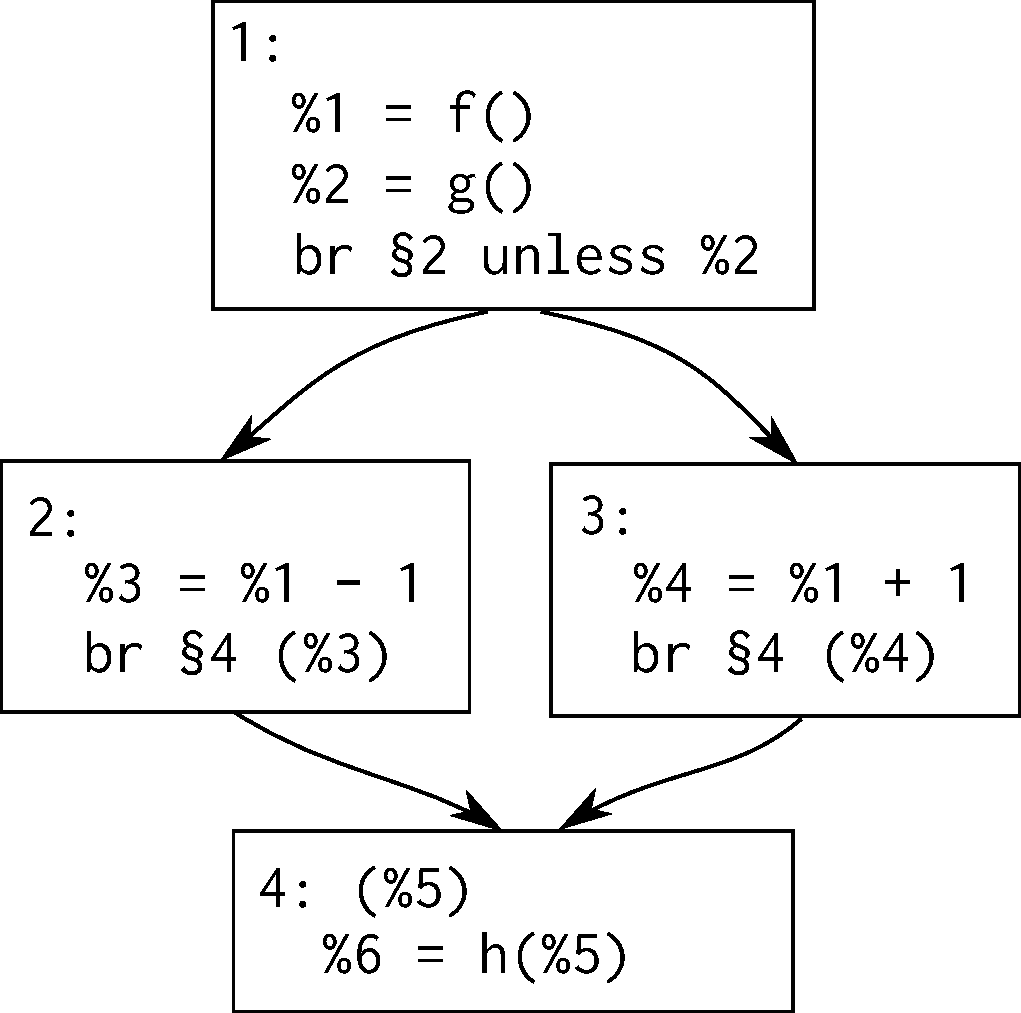
\includegraphics[width=0.4\textwidth]{figures/ssa-args}}
  \hfill\null
  \caption{Two control flow graphs of the same function, illustrating the correspondence between SSA
    representations using \(\phi\)-functions and block arguments.  The SSA variables
    \protect\jlinl{\%3} and \protect\jlinl{\%4} correspond to the values of \protect\jlinl{y} in the
    two branches, which are merged in \protect\jlinl{\%5}.}
  \label{fig:ssa-phi}
\end{figure}

Note that until now, the operations involved were purely syntactic in nature, and could be performed
by solely taking into account the code of the function \jlinl{foo}.  As soon as \jlinl{foo} is
called on a concrete type during evaluation, though, the most specific method fitting to the
argument types will be selected, and type inference on its body be applied.  If we go on and call
\jlinl{foo([1.0])}, with \jlinl{Vector\{Int\}} as the sole argument type, the types as annotated in
the same listing will be inferred.

\begin{lstfloat}[p]
  \begin{lstlisting}[style=lstfloat]
1 ── %1  = arraysize(x, 1)::Int64
│    %2  = slt_int(%1, 0)::Bool
│    %3  = ifelse(%2, 0, %1)::Int64
│    %4  = slt_int(%3, 1)::Bool
└───       goto §3 if not %4
2 ──       goto §4
3 ──       goto §4
4 ┄─ %8  = φ (§2 => true, §3 => false)::Bool
│    %9  = φ (§3 => 1)::Int64
│    %10 = φ (§3 => 1)::Int64
│    %11 = not_int(%8)::Bool
└───       goto §22 if not %11
5 ┄─ %13 = φ (§4 => 0.0, §21 => %18)::Float64
│    %14 = φ (§4 => %9, §21 => %42)::Int64
│    %15 = φ (§4 => %10, §21 => %43)::Int64
│    %16 = arrayref(true, x, %14)::Float64
│    %17 = invoke sin(%16::Float64)::Float64
│    %18 = add_float(%13, %17)::Float64
│    %19 = sle_int(1, 1)::Bool
└───       goto §7 if not %19
6 ── %21 = sle_int(1, 0)::Bool
└───       goto §8
7 ──       nothing::Nothing
8 ┄─ %24 = φ (§6 => %21, §7 => false)::Bool
└───       goto §10 if not %24
9 ──       invoke getindex(()::Tuple, 1::Int64)::Union{}
└───       $(Expr(:unreachable))::Union{}
10 ┄       goto §11
11 ─       goto §12
12 ─       goto §13
13 ─       goto §14
14 ─ %32 = invoke :(var"#sprint#339")(
             nothing::Nothing, 0::Int64, sprint::typeof(sprint), 
             show::Function, %18::Float64
           )::String
└───       goto §15
15 ─       goto §16
16 ─       goto §17
17 ─       invoke println("y += sin(x[i]) = "::String, %32::String)::Any
│    %37 = (%15 === %3)::Bool
└───       goto §19 if not %37
18 ─       goto §20
19 ─ %40 = add_int(%15, 1)::Int64
└───       goto §20
20 ┄ %42 = φ (§19 => %40)::Int64
│    %43 = φ (§19 => %40)::Int64
│    %44 = φ (§18 => true, §19 => false)::Bool
│    %45 = not_int(%44)::Bool
└───       goto §22 if not %45
21 ─       goto §5
22 ┄ %48 = φ (§20 => %18, §4 => 0.0)::Float64
└───       return %48
\end{lstlisting}
  \caption{Typed and optimized code of the call \protect\jlinl{foo([1.0])} in SSA form, as obtained
    through \protect\jlinl{@code_typed} (the extra bars are due to the formatting of
    \protect\jlinl{CodeInfo}).\label{lst:foo-typed}}
\end{lstfloat}

The last step of compilation within Julia consists of inlining and optimizing the typed intermediate
code, resulting in the form shown in listing~\ref{lst:foo-typed}.  There, several called methods
have been inlined, and concrete argument types to invoke been inferred.  This is in true,
traditional SSA form, with all variable slots eliminated, and block arguments converted to the
mentioned \(\phi\)-functions.  Finally, this representation will be translated and sent to LLVM for
compilation, where further optimization can happen, and machine code will be generated and executed,
as well as stored for later usage as part of the just-in-time compilation mechanism.

\newthought{A key principle} in Julia's compilation model is type specialization
\parencite{bezanson2018julia}.  As we have seen, whenever a function call is evaluated, the types of
the arguments are first determined, and then the most specific method selected and called.  This
automatically gives the language dynamic semantics: an implementation can perform evaluation at
every call.  In practice, however, at this point multiple dispatch and JIT compilation combine into
one of the main principles of optimization.  Instead of evaluating the same code over and over
again, methods are JIT-compiled the first time they are called.  The compiled code is then cached in
the method table.  Method compilation does not happen recursively at once, though.  Only when the
body of a compiled method is then executed with concrete arguments, the same process is performed
again, for each invoked method.

So, in a sense, JIT compilation can be seen as a function that returns compiled code, given a
function and a tuple of types.  Similar to macros, which transform original code, given an
expression, this process of generating compiled methods from types is customizable in Julia: via
so-called \emph{generated functions}, there exists a process to dynamically generate code, given
argument types~-- a form of staged programming
\parencite{rompf2010lightweight,bolewski2015staged}. Such generated functions, when called, are not
directly translated into machine code: instead, they emit new code to the compiler, based on the
types of their arguments.  The new code is then JIT-compiled.  For example, when we have two methods
of a function \jlinl{f}:
\begin{lstlisting}
f(x::Int) = println("Int")
f(x::String) = println("String")
\end{lstlisting}
we could replace them with the following generated function:
\begin{lstlisting}
@generated function f_generated(x)
    if x == Int
        return :(println("Int"))
    elseif x == String
        return :(println("String"))
    else
        error("Method error")
    end
end
\end{lstlisting}
Calling \jlinl{f_generated(1)} will then determine the argument type (\jlinl{typeof(1) == Int}), and
pass it to the function body of \jlinl{f_generated}.  There, the conditional will select the first
branch, and the expression \jlinl{:(println("Int"))} be returned.  This is now passed back to the
compiler, which will lower the code and compile the method for \jlinl{Int} arguments, and store the
result in the method table.  The stored code can then be executed~-- on the arguments that were used
to determine the type tuple the generated function has been called with!  The next time
\jlinl{f_generated} is executed, the function body is \emph{not} executed anymore, but the generated
code of the the function defined through the expression \jlinl{:(println("Int"))} directly looked
up\footnote{A caveat: technically, the compiler is still free to call the generating code multiple
  times~-- which is the reason generated functions should never involve side effects or depend on
  external state.}.  Of course, simply replacing dispatch, as with this example, is not what
generated functions are used for in practice.  Most applications concern parametric types with
statically known shape arguments, such as tuples, named tuples, or array ranks.  They can also be
used for type-level computations on values that become known only known at run-time, through
singleton types such as \jlinl{Val}.

The direct generation of code, given argument types, is however not the furthest we can go.  For
one, generated functions are not only allowed to return \jlinl{Expr} objects~-- the internal
representation of the surface AST~-- but also \jlinl{CodeInfo} objects, which are the internal
representation of lowered code in (almost) SSA form.  This, on its own, would not be of much use
most times, but there is a second, more interesting feature: it is possible to query the
\jlinl{CodeInfo} of a method by reflection, given a function and an argument type tuple.  Combining
these two, we now have all the tools to implement IR-level code transformations as follows:
\begin{enumerate}
  \firmlist
\item Define a generated function, taking as arguments another function and its arguments.
\item Within this function, obtain the IR of the method of the passed-in function for the remaining
  arguments.
\item Transform this IR however necessary.
\item Return the IR, which will now be compiled and called on the actual arguments.
\end{enumerate}
Importantly, unlike macros, such transformations can be performed \emph{recursively}: one simply
inserts the same generated function to inner function calls during the transformation in step 3.
Since the transformation operates not during parsing, the function to be transformed needs not be
known beforehand, and not be present literally in the code~-- the generated function can be called
on every available callable object, at any time during run-time.  This makes it possible to transform
even functions from other libraries, internally calling yet other functions.  One particular example
of this principle is source-to-source automatic differentiation, as shown in the next chapter: a
call to a function \jlinl{gradient(f, x, y)} will obtain the IR of the method for \jlinl{f} on
\jlinl{typeof(x)} and \jlinl{typeof(y)}, produce differentiated code, and call the result on
\jlinl{x} and \jlinl{y}.  Naturally, differentiating \jlinl{f} involves recursively differentiating
the other, unknown functions within it, too (down to \enquote{primitive} functions, whose derivative
is known), and combining the results using the chain rule.

This metaprogramming pattern is extremely powerful, and becoming more and more popular.  It allows
to change evaluation semantics in more profound ways than multiple dispatch can: by rewriting the
code of the called function, it is possible to change what invoking a method within its body means.
Through this, several abstract interpretation algorithms can be realized, by extending the existing
data path with additional metadata (such as automatic differentiation, or other forms of information
propagation analysis \parencite[part II]{singer2018static}), or non-standard execution be
implemented (e.g., continuation-passing style transformations).  There exist already two Julia
packages with the goal of simplify working with this kind of transformation:
\juliapackage{Cassette.jl}\footnote{\protect\url{https://github.com/jrevels/Cassette.jl}}, which
provides overloadable function application by a so-called \enquote{overdubbing} mechanism,
abstracting out some common patterns; and
\juliapackage{IRTools.jl}\footnote{\protect\url{https://github.com/FluxML/IRTools.jl}}, which has a
more user-friendly alternative to \jlinl{CodeInfo}, and a macro similar to \jlinl{@generated} that
makes writing recursive functional IR-transformation using this data structure easier.  The latter is
what the work of this thesis builds on.


%%%%%%%%%%%%%%%%%%%%%%%%%%%%%%%%%%%%%%%%%%%%%%%%%%%%%%%%%%%%%%%%%%%%%%%%%%%%%%%%%%%%%%%%%%%%%%%%%%%
\section[Automatic Differentiation and Computation Graphs]{Automatic Differentiation and \newline
  Computation Graphs}
\label{sec:cg-ad}

This section may appear as an outlier from the original topic; in fact, the mathematics developed
here are not even used later.  However, it is important to explain the interrelations between
automatic differentiation (AD), computation graphs, and IR transformations, to be able to understand
how SSA-form representation is a natural structure for extracting and analyzing computation graphs,
and how the necessary transformations arise in practice.  To appreciate how the form of the
computation graphs interacts with the mathematics, some foundations need to be introduced first.

\newthought{Many algorithms in machine learning} and other domains can be expressed as an
optimization problem over a multivariate function with scalar output~-- typically a loss function
over a parameter space, which measures how far a model prediction is form the true target values.
The optimal model is then just that one for which the parameters minimize the loss function.  When
the loss function is (sub-)differentiable, there exist a variety of gradient-based optimization
methods to find this optimum (or, in the non-convex case, at least a practically sufficient local
minimum).

While in some cases the loss function is simple enough to find the gradient by hand, in general, the
model, and therefore the loss function, may be specified in terms of rather complicated programs,
for which hand-writing derivatives is difficult to infeasible.  For this reason, computerized
methods for differentiation have been developed.  These can be categorized into three classes:
\begin{itemize}
  \firmlist
\item Finite differences
\item Symbolic differentiation
\item Automatic differentiation
\end{itemize}
In finite differences, the idea is to discretize the definition of derivatives, and numerically
evaluate the function within an environment.  This is simple to implement, but does not scale well
with the dimension of the involved space, and can become numerically unstable in various ways
\parencite[section 5.7]{press2007numerical}.  Symbolic differentiation works through representing
the functions in question as symbolic algebraic objects, and applying the differentiation rules as
one would manually.  This does not lose precision or introduce divergence, but can suffer from
blow-up of the size of the generated expressions; additionally, it requires the functions to be
expressed in a custom representation, different from normal functions or programs
\parencite{baydin2018automatic}.

\newthought{Automatic differentiation}, the third category, is perhaps unfortunately named~-- it
does not signify much at first sight.  The relevant idea is to not start from functions as black-box
or symbolic objects, but from programs.  Then the perturbation that makes up the value of the
derivative at a point is propagated through the steps of the program.  For this to work, there needs
to exist an explicit representation of the computation graph at  the evaluation at a point, which
is what makes the topic relevant for this thesis.  In contrast to the former two methods, AD relies
on numeric, not symbolic evaluation, but is (up to the floating point errors already present in the
input function) exact~-- no discretization error, as in finite differences, is introduced.  For a
more detailed treatment, I refer to \textcite{griewank2008evaluating}, the standard work on the
topic, and the survey by \textcite{baydin2018automatic}, which includes a comparison of
state-of-the-art implementations.  There are many works on the formalization of AD in programming
language theory; see, for example, \textcite{abadi2020simple}.

To understand how AD works, let us first start with the mathematics.  What is a derivative, really?
When we talk about gradients, which is what we really need in a gradient algorithm, this is usually
a rather informal term for \enquote{the vector of partial derivatives}, which then points into an
ascent direction.  This is however not the most natural form to work with in a compositional
approach.  Instead of starting with a limit of tangent slopes, more insight is provided by viewing
derivatives as best-approximating linear operators.  One of the most general definitions is provided
through the \emph{Fréchet derivative} \parencite[p. 463]{bronstein1995taschenbuch}, essentially a
generalization of the total differential.  Let \(X\) and \(Y\) be normed spaces.  A function
\(f: U \subseteq X \to Y\) is Fréchet differentiable at a point \(x \in U\) if there exists a
bounded linear operator \(A: X \to Y\) such that
\begin{equation}
  \label{eq:frechet}
  \lim_{\enVert{\Delta}_X \to 0} \frac{\enVert{f(x + \Delta) - f(x) -
      A(\Delta)}_Y}{\enVert{\Delta}_X} = 0.
\end{equation}
When such an \(A\) does exist, it is unique, and we may call it \emph{the} derivative of \(f\) at
\(x\), writing \(\Dif f(x) = A\).  When the derivative exists for all \(x\), we can use \(\Dif\) as
a well-defined higher-order function on its own; we will assume this in the following.\footnote{In
  in practical cases, functions are often only piecewise differentiable due to branches, failing
  this definition on a countable set of points.  Fortunately, the formalism of AD remains the same
  under weaker notions of differentiability.  Additionally, such points usually behave well enough
  to admit a subdifferential, from which we can just choose an arbitrary subgradient; this does not
  necessary lead to a descent direction, but still allows minimization under reasonable conditions
  \parencites[see][section 6.1]{pock2017convex}[][chapter
  14]{griewank2008evaluating}{abadi2020simple}.}

The important fact here is that \(\Dif f(x)\) is still a function: specifically, a linear function
approximating how \(f\) reacts to an input perturbation, \(\Delta\), around \(x\).  Or, in other
words:
\begin{equation}
  f(x + \Delta) = f(x) + \Dif f(x)(\Delta) + o\left(\enVert{\Delta}\right).
\end{equation}
This fact allows one to propagate differential values through composed functions, by the chain rule,
which we write in the following compositional form:
\begin{equation}
  \Dif(\phi \circ \psi)(x) = \Dif\phi(\psi(x)) \circ \Dif\psi(x).
\end{equation}
In the one-dimensional case, we simply have
\begin{equation}
  \Dif \phi(x) = \Delta \mapsto \partial_1 \phi(x) \, \Delta,
\end{equation}
where \(\partial_1 \phi(x)\) denotes the standard \enquote{primitive} derivative, since linear maps
are exactly multiplications by a scalar.  Therefore, we can recover the chain rule
\begin{equation}
  \begin{aligned}
    \Dif(\phi \circ \psi)(x)(\Delta) &=
    \left( \Dif\phi(\psi(x)) \circ \Dif\psi(x) \right)(\Delta) \\
    % &= \Dif\phi(\psi(x))\left( \Dif\psi(x)(\Delta) \right) \\
    % &= \Dif\phi(\psi(x))\left( \partial_1 \psi(x) \, \Delta \right) \\
    % &= \partial_1\phi(\psi(x)) \, \partial_1 \psi(x) \, \Delta \\
    &= \left( \partial_1\phi(\psi(x)) \, \partial_1 \psi(x) \right) \, \Delta,
  \end{aligned}
\end{equation}
as we know it from calculus.  Here, the product in the resulting expression arises from the fact
that we propagated through \(\partial_1 \psi(x) \Delta\) as the input value of
\(\Dif\phi(\psi(x))\).  It is, however, remarkable that this formula is not entirely compositional:
to construct \(\Dif(\phi \circ \psi)\), it is not only necessary to know \(\Dif\phi\) and
\(\Dif\psi\), but also \(\psi\) \parencite{elliott2018simple}.  Still, this is not as bad as it may
seem: as I will now explain, AD algorithms evaluate both \((\phi \circ \psi)(x)\) and
\(\Dif(\phi \circ \psi)(x)\) at once, in lockstep fashion, so that the intermediate values of the
former can be reused in calculation of the latter.

Consider the specific case of \(f(x, y) = sin(x) - y\). For simpler notation, let
\(g = (x, y) \mapsto x - y\) replace the infix subtraction operator, with a derivative of
\(\Dif g(x)(\Delta_1, \Delta_2) = \Delta_1 - \Delta_2\).  By composition, we have:
\begin{equation}
  \begin{aligned}
    \Dif f(x, y) &= \Dif(g \circ (\sin \otimes \ident))(x, y) \\
    &= \Dif g\left( (\sin \otimes \ident)(x, y) \right) \circ \Dif(\sin \otimes \ident)(x, y) \\
    % &= \left( (\Delta_1, \Delta_2) \mapsto \Delta_1 - \Delta_2 \right) \circ \left( \Dif\sin(x)
      % \otimes \Dif \ident(y) \right) \\
    % &= (\Delta_1, \Delta_2) \mapsto \partial_1\sin(x) \, \Delta_1 - 1 \Delta_2 \\
    &= (\Delta_1, \Delta_2) \mapsto \cos(x) \, \Delta_1 - \Delta_2.
  \end{aligned}
\end{equation}
In order to calculate this algorithmically, let us expand the computation of \(f\) into a sequence
of intermediate, primitive calculations, as we would have in a programmatical representation:
\begin{equation}
  \label{eq:ad-primal}
  \begin{aligned}
    x &= \operatorname{?}, \\
    y &= \operatorname{?}, \\
    z &= \sin(x), \\
    \Omega &= g(z, y).
  \end{aligned}
\end{equation}
We have given the final result the name \(\Omega\), and and introduced an intermediate value \(z\).
This is known as the \emph{forward}, or \emph{primal} function in AD terminology.  The relations of
these values can be expressed as the black computation graph in figure~\ref{fig:comp-graph-fw}.
Following the graph, or equivalently, following the equations in ~\eqref{eq:ad-primal}, the
composition of the derivative operators can be built up incrementally, as shown in the blue part of
that figure, by calculating the following \emph{tangent values}:
\begin{equation}
  \label{eq:ad-forward}
  \begin{aligned}
    \dot{x} &= \Delta_1, \\
    \dot{y} &= \Delta_2, \\
    \dot{z} &= \Dif\sin(x)(\dot{x}) \\
    &= \cos(x) \, \Delta_1, \\
    \dot{\Omega} &= \Dif g(z, y)(\dot{z}, \dot{y}) \\
    &= \cos(x) \, \Delta_1 - \Delta_2.
  \end{aligned}
\end{equation}
The tangent values of input variables \(x\) and \(y\) become the input perturbations \(\Delta_i\).
For every subsequent tangent value, we apply the derivative at the corresponding primal variable
(depending on the primal parents) to the tangent values of the parents~-- this way, the composition
of the derivative operators follows the chain rule.  This algorithm, called \emph{forward-mode AD},
can now be applied practically not only on symbolic functions, but on programs, by always jointly
computing \((v, \dot{v})\) for every variable \(v\), given its parents in the graph.  This requires
a form of non-standard execution, which will be explained in more detail below.

\begin{figure}[t]
  \centering
  \subbottom[Forward mode.\label{fig:comp-graph-fw}]{%
    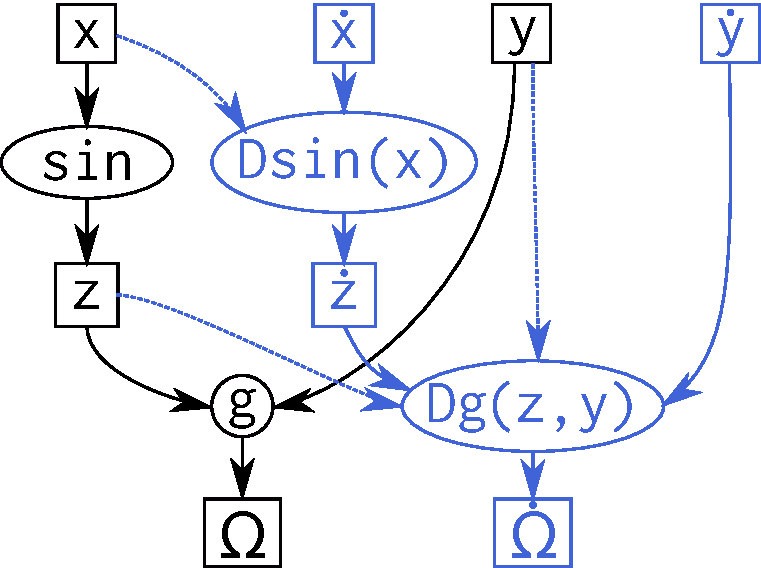
\includegraphics[]{figures/comp-graph}}
  \qquad
  \subbottom[Backward mode.\label{fig:comp-graph-bw}]{%
    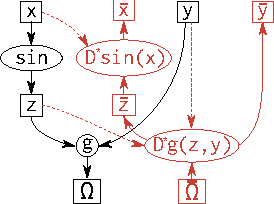
\includegraphics[]{figures/comp-graph-backward}}
  \caption{Computation graph and intermediate expressions of the expression \protect\jlinl{g(sin(x),
      y)}, together with the derivative graphs in forward- and backward mode.  Dashed arrows
    indicate re-use of primal values in the derivative graph.}
  \label{fig:comp-graph}
\end{figure}

\newthought{Recovering the full gradient} of a function \(\phi: U \subseteq \RR^N \to \RR\) (which
is generally the form of loss functions for parametric models) requires to evaluate \(\Dif \phi(x)\)
\(N\) times, however.  This is because individual partial derivatives can only be extracted from
\(\Dif \phi(x)\) by calculating the sensitivities to unit input perturbations in coordinate
directions, for each of the input variables:
\begin{equation}
  \nabla \phi(x) = \begin{pmatrix}
    \Dif \phi(x)(1, 0, \ldots, 0)  \\
    \vdots \\
    \Dif \phi(x)(0, \ldots, 0, 1)
  \end{pmatrix} = \begin{pmatrix}
    \partial_1 \phi(x) \\
    \vdots \\
    \partial_N \phi(x)
  \end{pmatrix},
\end{equation}
which is really a special case of taking directional derivatives (which can be recovered generally
by application of the differential to any vector with unit norm.)

In order to overcome the increase of complexity with the number of input dimensions, we can
reformulate the compositional equation.  Let us introduce \(\CoDif \phi(x)\), the \emph{adjoint
  operator} of \(\Dif \phi(x)\), whose defining property is that in \enquote{inverts} the order of
the perturbation application: instead of calculating a primal sensitivity with respect to an input
perturbation (\(\Delta\)), it maps a linear output perturbation (\(\mathfrak{d}\)) to an operator
that applies this to the primal sensitivity:
\begin{equation}
  \CoDif \phi(x)(\mathfrak{d}) = \Delta \mapsto \mathfrak{d}(\Dif \phi(x)(\Delta)).
\end{equation}
The adjoint differential is therefore an object of the double dual space.  This becomes more
readable when we fix a basis to represent the derivative.  Doing so, in the finite-dimensional case,
the derivative \(\Dif \phi(x)\) is the Jacobian matrix at \(x\), \(J_{\phi}(x)\).  In this setting,
forward-mode AD is simply an efficient way to calculate the \emph{Jacobian-vector-product}
\(J_{\phi}(x) \Delta\), or equivalently the total derivative for a fixed perturbation, avoiding full
matrix multiplication~-- which is the reason we have to apply it to the basis vectors to get back
the gradient.  Backward mode, on the other hand, calculates the product of the Jacobian with the
operator that should be applied to the result, but does not yet apply it to the input
perturbation~-- therefore, it returns a matrix:
\begin{equation}
  \begin{aligned}
    \mathfrak{d} (\Dif \phi(x)(\Delta)) &= \transpose{d} J_{\phi}(x) \Delta \\
    &= \transpose{\left( \transpose{J_{\phi}(x)} d \right)} \Delta \\
    &= \CoDif \phi(x)(\mathfrak{d})(\Delta),
  \end{aligned}
\end{equation}
where we assume \(\mathfrak{d}\) to be represented by the co-vector \(\transpose{d}\).  Since the
unapplied \(\CoDif \phi(x)(\mathfrak{d})\) is itself an object in the dual space, it is also
represented as a co-vector~-- and in fact, nothing else than a transformation of the transposed
Jacobian.  Recovering the gradient of a loss function then reduces to evaluating it at a constant
scalar output perturbation of \(1\), which is equivalent to the application of the primal
differential to the matrix of basis vectors.

Note that due to this relation to the transpose, the adjoint operator inverses the order of
composition in the chain rule:
\begin{equation}
  \begin{aligned}
    \CoDif (\phi \circ \psi)(x)(\mathfrak{d}) &= \transpose{d} J_{\phi}(\psi(x)) J_{\psi}(x) \\
    &=  \transpose{\left( \transpose{J_{\psi}(x)} \transpose{J_{\phi}(\psi(x))} d \right)} \\
    &= \left( \CoDif\psi(x) \circ \CoDif\phi(\psi(x)) \right)(\mathfrak{d}).
  \end{aligned}
\end{equation}
For our example function \(f\), this gives the same structural form of the result as the forward
mode~-- only that now, the value is a vector:
\begin{equation}
  \begin{aligned}
    \CoDif f(x, y) &= \CoDif (g \circ (\sin \otimes \ident))(x, y) \\
    &= \CoDif(\sin \otimes \ident) \circ \CoDif g((\sin \otimes \ident)(x, y)) \\
    % &= (\CoDif\sin \otimes \CoDif\ident) \circ (\delta \mapsto \transpose{[\delta, -\delta]}) \\
    % &= (\partial_1 \sin(x) \otimes 1) \circ (\delta \mapsto \transpose{[\delta, -\delta]}) \\
    % &= \delta \mapsto \transpose{[\partial_1\sin(x)\delta, -1 \delta]} \\
    &= \delta \mapsto \transpose{[\cos(x)\delta, -\delta]}.
  \end{aligned}
\end{equation}
In this form, starting with an output perturbation \(\delta = 1\), we get back the gradient tuple
through just one evaluation.  Incidentally, this is nothing else than the back-propagation
\enquote{trick} \parencite{bishop2006pattern}!  Furthermore, applying this result to
\([\Delta_1, \Delta_2]\) gives back the linear combination of the forward mode result.

In programmatic terms, we can proceed similar to above, only this time introducing \emph{adjoint}
intermediate values \(\bar{v}\).  For the values in equation~\eqref{eq:ad-primal}, we get
\begin{equation}
  \label{eq:ad-backward}
  \begin{aligned}
    \bar{x} &= \bar{z}_2 = -\delta, \\
    \bar{y} &= \CoDif\sin(x) \, \bar{z}_1 \\
    &= \cos(x) \, \delta\\
    \bar{z} &= \CoDif g(x, y)(\bar{\Omega}) \\
    &= [\delta, -\delta] \\
    \bar{\Omega} &= \delta,
  \end{aligned}
\end{equation}
which is displayed in the red graph in \ref{fig:comp-graph-bw}.  Note that now, the back-propagated
values can not be computed in parallel with forward evaluation; hence the equations are stated in
reverse order.  Instead, the intermediate primal values have to be remembered and reused in a
second, backward pass.

Finally, it has to be noted that the two described modes of automatic differentiation are only two
extremes of a spectrum.  Forward and backward calculations can really be interleaved in arbitrary
order, just as it is possible to multiply Jacobians and their transposes in different order.  One
frequent use case of this \emph{mixed-mode AD} is when loss functions, differentiated using backward
mode, contain broadcasting functions; for example, nonlinearities in neural network.  These have a
shape of \(\RR^N \to \RR^N\), but only involve a linear number of operations, so forward mode pays
off\footnote{As a rule of thumb in Julia, for \(f: \RR^M \to \RR^N\), forward mode typically
  performs better when \(M \ll N\) or as long as \(M \lessapprox 100\).  This folklore should always
  be confirmed by benchmarking, though.  See
  \url{https://github.com/JuliaDiff/ReverseDiff.jl\#should-i-use-reversediff-or-forwarddiff}.}.
Similar properties hold for second order derivatives: the calculation of Hessians is often fastest
by using forward-over-reverse composed differentiation.  In general, unfortunately, determining the
optimal order of derivative evaluation is hard~-- this so-called \emph{optimal Jacobian
  accumulation} problem is known to be NP-complete \parencite{naumann2007optimal}.

\newthought{The practical implementation} of automatic differentiation in programming languages
opens up another set of possible choices.  One way is to use an external, compiler-based system that
transforms a complete program in a subset of a standard programming language (e.g., Tapenade, which
transpiles Fortran and C code \parencite{tapenadedevelopers2019tapenade}) or in a custom
specification, as is done in Stan \parencite{carpenter2015stan}.  But both of these examples are
really applied in niche cases: large numeric simulations, and log-densities in a probabilistic
model.  These systems lack flexibility in programming, especially concerning abstractions and
interaction with other libraries, and require external tooling besides a main programming language.
Recently, the Swift for TensorFlow project \parencite{tensorflowdevelopers2018swift,hong2018graph}
introduced a modern variant of this by extending the compiler of the Swift programming language with
facilities to perform automatic differentiation internally, and some features to simplify graph
operations required by TensorFlow.

The second possibility is \emph{operator overloading}.  Forward mode can be recast in mathematically
equivalent form by using dual numbers \parencite[see][section 3.1.1]{baydin2018automatic}.  These
consist of two parts, similar to complex numbers: \(z = x + y\epsilon\).  However, contrary to the
imaginary unit, the infinitesimal unit \(\epsilon\) vanishes under multiplication with itself:
\(\epsilon^2 = 0\).  The consequence of this is that functions can naturally be extended to dual
numbers by nonstandard interpretation as truncated Taylor series:
\begin{equation}
  \phi(x + \epsilon) = \phi(x) + \partial_1\phi(x)\epsilon + \underbrace{\frac{\partial^2_1\phi(x)}{2}\epsilon^2
  + \ldots}_{\epsilon^2 (\ldots) = 0}
\end{equation}
Since the higher order terms vanish, this is exactly the tuple of primal and tangent value that is
calculated during the lockstep evaluation in forward mode:
\begin{equation}
  (z, \dot{z}) = (\phi(x), \Dif\phi(x)(\dot{x})) \quad\Leftrightarrow\quad z + \dot{z}\epsilon = \phi(x + \dot{x}\epsilon).
\end{equation}
(generalization to higher dimensions, as well as higher derivatives in form of hyper-dual numbers,
follow equally naturally.)

Dual numbers can rather easily be added to an existing programming language that has a sufficiently
extensible system for overloading mathematical operators.  This can be done using traits or type
classes, like in Haskell, or by dynamic dispatch, which is what is used in Python and Julia.  The
latter is especially versatile in this respect, since every function can be extended to a new type
of dual numbers by simply adding a method; unlike in Python, where only certain operators are open
to extension~-- a fundamental limitation of its single dispatch, object oriented approach.

\begin{figure}[t]
  \centering
  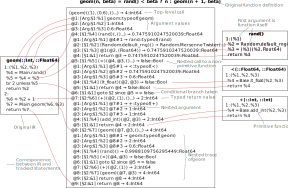
\includegraphics{figures/wengert-list}
  \caption{Wengert list of the example function \protect\jlinl{g(sin(x), y)} introduced above.
    Every intermediate variable becomes an element, linked through pointers.  The gradient can be
    calculated by backward traversal and accumulating the adjoint values as metadata in the list
    elements.}
  \label{fig:wengert-list}
\end{figure}

Backward-mode AD can be implemented using operator overloading as well, but this requires more
effort.  Since adjoint values cannot be simply threaded through in parallel to forward evaluation,
one needs to build up a data structure during the forward pass, which can at the end be traced back
in reverse order.  One possibility of doing this is to use closures, but the usage of many higher
order function might lead to unwanted heap allocation and makes understanding harder.

The alternative is to use a tape structure, or \emph{Wengert list} \parencite[][section
3]{baydin2018automatic}.  On such a list, the computation graph is stored as by pointers between
elements, as shown in figure~\ref{fig:wengert-list}.  The Wengert list can also be constructed
through an operator overloading approach, which is exactly what graph-based machine learning
frameworks do: PyTorch \parencite{paszke2017automatic}, TensorFlow \parencite{abadi2015tensorflow}
in eager mode, DyNet \parencite{neubig2017dynet}, and Chainer \parencite{tokui2015chainer}.  In
these, the programmer interacts with a library mirroring the usual numerical functions, but
operating on a special \enquote{variable} or \enquote{tensor} type.  These operations are overloaded
so that function calls, in addition to performing the primal calculations, are stored either
explicitly on a global Wengert list structure, or implicitly in the constructed expression objects.
Then, one can start a backward pass from any leaf variable to propagate back derivatives to the
roots of the computation graph, by following the edges and summing up adjoint values in parent
nodes' metadata.  JAX \parencite{bradbury2018jax} carries the idea further and allows general
composable source transformations to implement not only differentiation, but also vectorization,
parallelization, and other syntactic abstractions over functional programs written in Python, over a
unified intermediate representation that is recovered from an original function by tracing.

This style of implementation has limitations, though: it requires building up many objects at
run-time, and is completely oblivious of control structures.  Additionally, the code expressing
differentiable functions has to be written entirely in the DSL, in a library-aware fashion,
preventing the usage of third-party functions and language features, and forcing the user to adhere
to certain semantic constraints that cannot be verified statically by the host language.  TensorFlow
in graph mode addresses some of these points.  It builds up a complete expression graph, which is
differentiated symbolically, and is therefore somewhat in the middle between operator overloading
(since the graph is still a run-time data structure) and a static transformation (the resulting graph
is not interpreted in the host language, but converted to run on an \enquote{accelerator}, which can
one of several kinds of processing unit~-- CPU, GPU, TPU,\ldots).  It still requires to stick to the
provided expression types and library functions, though.

Efforts to overcome these limitations lead to the third kind of approach: language-internal
\emph{source transformation}.  Recent work in Julia \parencite{innes2018don} has shown that through
the available metaprogramming mechanisms (described in section~\ref{sec:comp-metapr-julia}) allow to
systematically derive \enquote{adjoint programs} for arbitrary user-provided Julia functions, given
only an extensible set of \emph{primitive adjoints}.  This approach works purely structurally on the
Julia IR, employing generated functions to analyze functions' code and transform them completely,
including third-party functions and data types, and control flow.  The key insight here is that
SSA-form IR already resembles the structure of Wengert lists, extended by branches.  As in building
up reverse computation graphs, the adjoint code will therefore invert the control flow of the basic
blocks in the primal function, taking into account that data flow may involve dynamic dependencies.
Differentiation through data types and closures is supported via a unified treatment of them in a
tuple-like form, with constructors and accessors (inspired by cons-cells in Lisp).

An implementation of this principle has been released as the \juliapackage{Zygote.jl}
package\footnote{\url{https://github.com/FluxML/Zygote.jl}}.  In similar spirit, there is also work
on directly differentiating the LLVM intermediate representation, by extending the compiler pipeline
with a differentiation pass that comes after all language-specific and high-level optimizations
\parencite{moses2020instead}.  Furthermore, there are applications that use the same techniques for
other purposes, like sparsity detection \parencite{gowda2019sparsity} or concolic execution
\parencite{churavy2019vchuravy}.

Internal source-based methods can therefore be composable, extensible, and more user-friendly, since
no special treatment of programs to be differentiated is required: primal functions can be
implemented as any other regular function in the host language.  A source-transformation approach
also completely avoids the obscure issue of \enquote{perturbation confusion}, which leads to
hard-to-find errors when using nested differentiation with dual numbers
\parencite{baydin2018automatic,manzyuk2019perturbation}.

As a concluding note, all these graph operations reveal that automatic differentiation is really
only a special case of message passing algorithms in computation graphs
\parencite{minka2019automatic}.  Other learning methods that can be described as message passing are
optimization algorithms \parencite{ruozzi2011message,dauwels2005steepest} and a variety of
variational approximations \parencite{winn2005variational,minka2005divergence}.  Hence, it is no
surprise that computation graphs play a large role as the foundation of other learning algorithms in
Bayesian methods, such as described below.

%%% Local Variables: 
%%% TeX-master: "main"
%%% End: